\documentclass[a4paper,rep]{thesisby}

\usepackage[T2A]{fontenc}
\usepackage[utf8]{inputenc}
\usepackage[english, russian]{babel}
\usepackage{lastpage}

\usepackage{amsmath, amssymb, amsfonts}
\usepackage{longtable,array}
\usepackage{fixltx2e}
\usepackage{multirow}

\usepackage{afterpage}

\usepackage{algorithmic}
\usepackage{algorithm}


\usepackage{color}


\emergencystretch=25pt

\newcommand{\abs}[1]{\left\vert#1\right\vert}
\renewcommand{\theequation}{\arabic{equation}}
\renewcommand{\thefigure}{\arabic{figure}}
\renewcommand{\thetable}{\arabic{table}}
\renewcommand{\labelenumii}{\arabic{enumii}}

\newcommand*{\mbb}{\mathbb}
\newcommand*{\mbf}{\mathbf}

\newcommand*{\diff}{\mathop{}\!\mathrm{d}}% Differential
\newcommand*{\pd}{\partial}% Partial differential
\newcommand*{\im}{\ensuremath{\mathrm{i}}}% Imaginary unit
\newcommand*{\e}{\mathop{\mathrm{e}}\nolimits}% The number "e"
\newcommand*{\const}{\ensuremath{\mathrm{const}}}% const
\DeclareMathOperator{\diverg}{div}% Divergence

\newcommand*{\Four}{\mathcal{F}}%{\hat}% Fourier transform
\newcommand*{\Lapl}{\mathcal{L}}%{\tilde}% Laplace transform
\newcommand*{\ctrw}{\mathrm{RW}}
\newcommand*{\dctrw}{\mathrm{DRW}}
\newcommand*{\drwg}{\mathrm{DRWG}}
\newcommand*{\drwb}{\mathrm{DRWB}}
\newcommand*{\te}{\mathrm{TE}}
\newcommand*{\de}{\mathrm{DE}}
\newcommand*{\Gauss}{\mathrm{G}}
\newcommand*{\Bern}{\mathrm{B}}
\newcommand*{\discr}{\mathrm{d}}
\newcommand*{\singul}{\mathrm{s}}
\newcommand*{\regul}{\mathrm{r}}

\newcommand{\Rb}{\mathbb R}
\DeclareMathOperator{\dist}{dist} \DeclareMathOperator{\diam}{diam}

\newcommand{\diffd}[2]{\frac{\partial^2}{\partial #1 \partial #2}}
\newcommand{\sumd}[2]{\sum_{u = #1}^{#2}}
\newcommand{\ceilr}{\lceil r \rceil}
\newcommand{\floor}[1]{\lfloor #1 \rfloor}
\newcommand{\enbrace}[1]{\lb #1 \rb}
\newcommand{\inv}[1]{{#1}^{-1}}
\newcommand{\setdef}[2]{\left\{ #1\ \left|\ #2 \right.\right\}}
\newcommand{\seqz}[2]{\left\{ {#1}_{#2} \right\}_{#2\in\Zb}}
\newcommand{\seq}[1]{ \{ #1 \} }
\newcommand{\half}[1]{\frac{#1}{2}}
\newcommand{\vmod}[1]{\left| #1 \right|}
\newcommand{\Ah}{\hat{A}}
\newcommand{\No}{\textnumero}

\usepackage{graphicx}
\usepackage{epstopdf}

\textwidth=170mm \textheight=240mm

\makeatletter
\renewcommand\@biblabel[1]{#1 }
\makeatother

\DeclareMathSymbol{\Pi}{\mathalpha}{letters}{"05}

\begin{document}

%!TEX root = stoh_modeling.tex
\begin{titlepage}

\begin{center} %\bfseries
{%\fontsize{14.4pt}{4mm}\selectfont
%\large
Министерство образования и науки Российской Федерации\\
%\medskip
Федеральное государственное автономное образовательное учреждение\\
высшего образования\\
<<Санкт-Петербургский политехнический университет Петра Великого>>
}
\end{center}
\vspace{0.5cm}

\hspace{-5mm}
\begin{tabular}{lcr}
{
	\begin{tabular}[t]{l}
		УДК\\
		\No{} \\
		Инв. \No{} \\
	\end{tabular}
} & \hspace{40mm} & {
	\begin{tabular}[t]{l}
		У Т В Е Р Ж Д А Ю \\
		Зав. НИЛ <<Математическая биология\\
		и биоинформатика>>, ИПММ\\
		ФГАОУ ВО <<СПбПУ>>,\\
		д.б.н. \\
		\underline{\hspace{4cm}} М. Г. Самсонова\\
		<<\underline{\hspace{1cm}}>> \underline{\hspace{3cm}} 2016 г.
	\end{tabular}
}\\
\end{tabular}
\vspace{2cm}



\begin{center}
{%\bfseries
%\large
ОТЧЕТ\\
О НАУЧНО-ИССЛЕДОВАТЕЛЬСНОЙ РАБОТЕ\\
\vspace{3mm}
по теме:\\
<<Стохастическое моделирование экспрессии генов>>\\
}
\end{center}

\vspace{1.5cm}


\hspace{15mm}
\begin{tabular}{ll}
{
	\hspace{60mm}
}&{
	\begin{tabular}[t]{l}
		Выполнил студент гр. \No{53601/4}\\
		{}\\
		\underline{\hspace{2cm}} Д. В. Яковлев\\
		<<\underline{\hspace{1cm}}>> \underline{\hspace{3cm}} 2016 г.
	\end{tabular}
}\\
{
	{}
}&{
}\\
{
	{}
}&{
	\begin{tabular}[t]{l}
		Руководитель НИР, к.ф.-м.н. \qquad\\
		{}\\
		\underline{\hspace{2cm}} В.В. Гурский \\
		<<\underline{\hspace{1cm}}>> \underline{\hspace{3cm}} 2016 г.
	\end{tabular}
}\\
\end{tabular}
\vspace{20mm}

\begin{center}
 %\large
 Санкт-Петербург 2016
\end{center}

\end{titlepage}


\newpage
%!TEX root = stoh_modeling.tex
\section*{РЕФЕРАТ}
Отчёт 14 стр., 1 часть, 5 рис., 5 источников

СТОХАСТИЧЕСКОЕ МОДЕЛИРОВАНИЕ ЭКСПРЕССИИ ГЕНОВ
В данной работе описываются реакции моделирования экспрессии генов. Приводятся результаты стохастического моделирования экспрессии генов.


\newpage
\tableofcontents


\newpage
%!TEX root = stoh_modeling.tex
\section*{Введение}
\addcontentsline{toc}{section}{Введение}
Цель научноисследовательской работы:
\begin{itemize}
    \item Описать реакции экспресии генов
    \item Разработка программного обеспечения для стохастического моделирования
    экспресии генов.
    \item Анализ экспериментальных рассчётов
    \item Выводы
\end{itemize}


\newpage
%!TEX root = stoh_modeling.tex
\section{Постановка задачи}
Время работы алгоритма попарного выравнивания, основанного на динамическом заполнении матрицы выравниваний можно оценить как $O(n^2)$, где $n$ - максимально возможное количество разрезов на карте. Целью данной работы является описание и исследование двух эвристических методов, которые позволяют его ускорить, и добиться оценки среднего времени работы $O(n)$ для каждого из них. В данной работе будет проведено сравнение двух этих методов между собой и с исходным алгоритмом. Будет показано, что использование этих методов предпочтительно в случае определенной модели структуры множества исходных рестрикционных карт, а так же будут оценены границы применимости данных эвристик.


\newpage
%!TEX root = stoh_modeling.tex
\section{Результаты}
\subsection{Процесс моделирования}
\subsection{Экспериментальные расчёты}
\begin{figure}[h]
 	\center{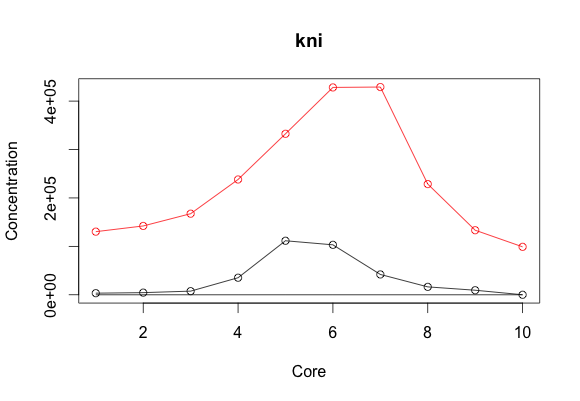
\includegraphics[width=1\linewidth]{kni}}
\end{figure}
\begin{figure}[h]
 	\center{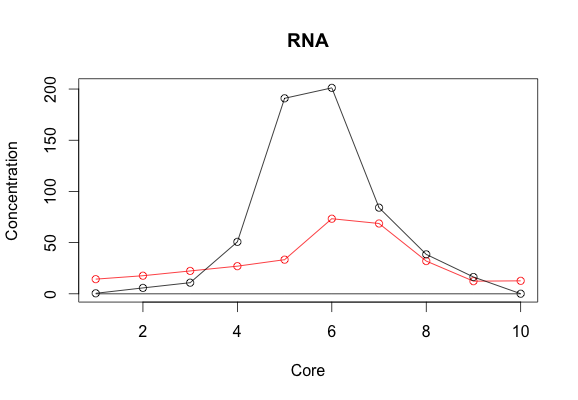
\includegraphics[width=1\linewidth]{rna}}
\end{figure}


\newpage
\chapter*{Выводы}

\newpage
\bibliographystyle{utf8gost71u}
\bibliography{biblio}

\end{document}
